%------------------------------------------%
% Cannabis Data Science
% Date: 1/5/2022
%------------------------------------------%
\documentclass[xcolor={dvipsnames}]{beamer}
\hypersetup{pdfpagemode=FullScreen}
\mode<presentation>{
  \usetheme{Boadilla}
  \usecolortheme{orchid}
  \usefonttheme{default}
  \setbeamertemplate{navigation symbols}{}
  \setbeamertemplate{caption}[numbered]
} 
\usepackage[english]{babel}
\usepackage[utf8x]{inputenc}
\setbeamersize{text margin left=0.5in,text margin right=0.5in}

\usepackage[dvipsnames]{xcolor}
\definecolor{DarkGreen}{RGB}{2, 48, 32}
\definecolor{CalyxGreen}{RGB}{34, 153, 84}
\definecolor{DarkOrange}{RGB}{199, 0, 57}
\definecolor{LightOrange}{RGB}{255, 87, 51}
\definecolor{LightGreen}{RGB}{218, 247, 166}
\definecolor{LightYellow}{RGB}{255, 195, 0}

\setbeamercolor*{palette primary}{bg=LightGreen, fg = DarkGreen}
\setbeamercolor*{palette secondary}{bg=LightGreen, fg=DarkGreen}
\setbeamercolor*{palette tertiary}{bg=LightGreen, fg = DarkGreen}
%\setbeamercolor*{palette quaternary}{bg=myNewColorD, fg = green}

%------------------------------------------%
% Packages
%------------------------------------------%
\usepackage{amsmath}
\renewcommand*\footnoterule{} %No sperating line on footnote
\usepackage{mathtools} %ANNOTATING EQUATIONS
\usepackage{hhline} %DOUBLBARS
\usepackage[super]{nth}
\usepackage{graphicx, caption, subcaption}

%------------------------------------------%
% Commands
%------------------------------------------%
\newcommand\T{\rule{0pt}{2.5ex}} %TOPSTRUT
\newcommand\B{\rule[-1.25ex]{0pt}{0pt}} %BOTTOMSTRUT
\newenvironment<>{varblock}[2][.9\textwidth] %RESIZED BLOCKS
  {\setlength{\textwidth}{#1}
  \begin{actionenv}#3
    \def\insertblocktitle{#2}\par
    \usebeamertemplate{block begin}}
  {\par\usebeamertemplate{block end}
  \end{actionenv}}
\defbeamertemplate{enumerate item}{largeball} %LARGE BALLS
{\begin{pgfpicture}{-1ex}{-0.65ex}{1.5ex}{1.5ex}
\usebeamercolor[fg]{item projected}
{\pgftransformscale{2.5}\pgftext{\Large\pgfuseshading{bigsphere}}}
{\pgftransformshift{\pgfpoint{0pt}{0.5pt}}
\pgftext{\usebeamerfont*{item projected}\small\insertenumlabel}}
\end{pgfpicture}}
\usepackage{tikz} % FANCY ARROWS
\usepackage{xparse}
\NewDocumentCommand\UpArrow{O{2.0ex} O{black}}{%
   \mathrel{\tikz[baseline] \draw [->, line width=0.5pt, #2] (0,0) -- ++(0,#1);}} % FANCY UPARROW
\NewDocumentCommand\DownArrow{O{2.0ex} O{black}}{%
   \mathrel{\tikz[baseline] \draw [<-, line width=0.5pt, #2] (0,0) -- ++(0,#1);}} % FANCY DOWNARROW
%\vskip 1cm
\makeatletter
\newcommand{\LeftEqNo}{\let\veqno\@@leqno}%LEFT EQUATION #'s
\makeatother

%------------------------------------------%
% Title
%------------------------------------------%
\title[\textbf{Meetup}]{}
\author{Cannabis Data Science}
\institute[]{\Large Meetup}
\date{January \nth{5}, 2022}
\begin{document}
\begin{frame}{}
  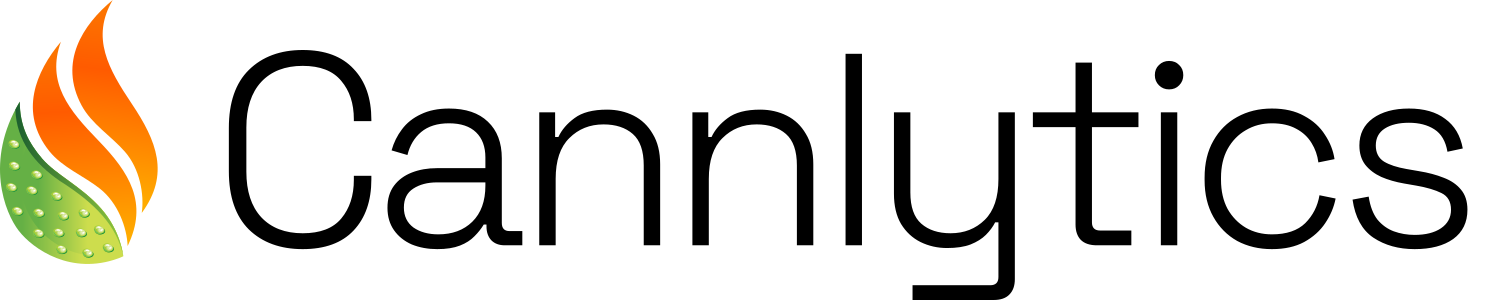
\includegraphics[scale=0.075]{images/logos/cannlytics_logo_with_text_light.png}
  \titlepage
\end{frame}

%------------------------------------------%
% Introduction
%------------------------------------------%
\section{Introduction}

% Data Science Pioneers
\begin{frame}{}

{\large \textbf{Data Science Pioneers}}\vspace{0.5\baselineskip}\\

% Images of data science pioneers
\begin{figure}
    \begin{subfigure}[t]{.425\textwidth}
      \begin{center}
      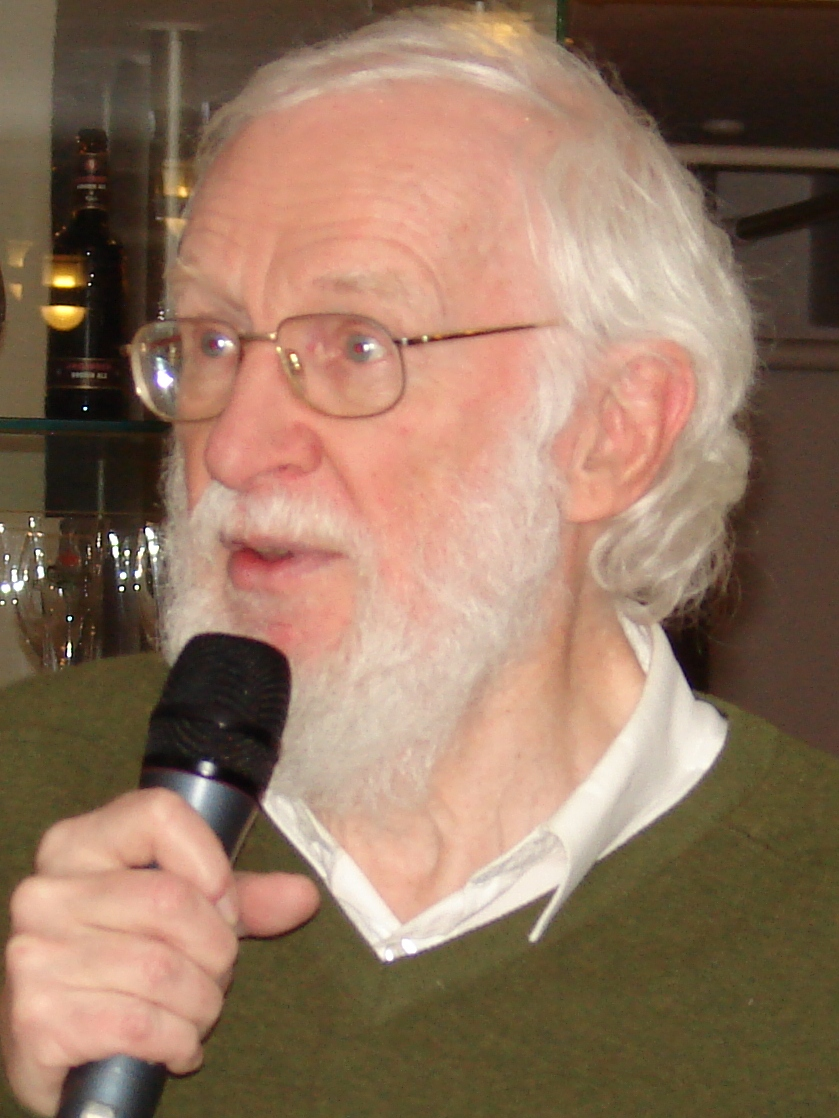
\includegraphics[height=4cm]{images/Peternaur.jpg}
      \end{center}
      \caption*{\textbf{Peter Naur} - Began using ``\textit{data science}'' as an alternative name for computer science as early as 1974.\vspace{0.5\baselineskip}\\ \tiny Author: Eriktj at English Wikipedia\newline CC BY-SA 3.0\newline https://creativecommons.org/licenses/by-sa/3.0/\newline No changes were made to the image.}
    \end{subfigure}%
    \hspace{.075\textwidth}
    \begin{subfigure}[t]{.425\textwidth}
      \begin{center}
      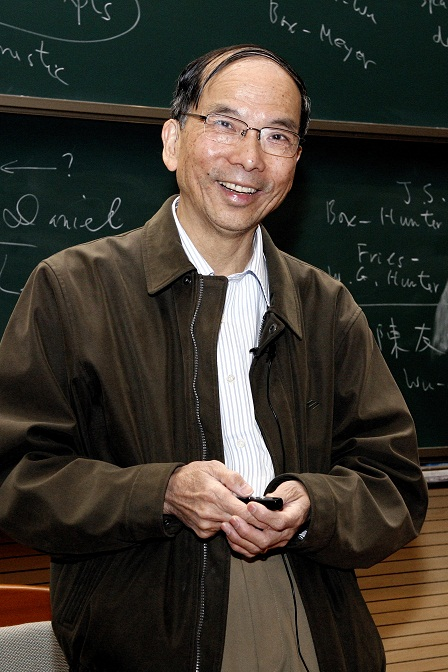
\includegraphics[height=4cm]{images/C.F._Jeff_Wu_at_Chinese_Academy_of_Sciences_2011.jpg}
      \end{center}
      \caption*{\textbf{C.F. Jeff Wu} - Used ``\textit{data science}'' as an alternative name for statistics in 1985.\vspace{0.5\baselineskip}\\ \tiny Commissioned by the owner, C. F. Jeff Wu\newline CC BY-SA 3.0\newline https://creativecommons.org/licenses/by-sa/3.0)\newline No changes were made to the image.}
    \end{subfigure}
\end{figure}

\end{frame}

% About Data Science
\begin{frame}{}


{\large Latanya Sweeney (Harvard Professor)has suggested 3 trends in data science:}\vspace{1.5\baselineskip}\\

\begin{itemize}

\item \textbf{Collect more} - Expansion of the number of fields being collected.

\vspace{1\baselineskip}

\item \textbf{Collect specifically} - Replace an existing aggregate data collection with a person-specific one.

\vspace{1\baselineskip}

\item \textbf{Collect it if you can} - Gather information by starting a new person-specific data collection.

\end{itemize}

\end{frame}

% The Data Deluge
\begin{frame}{}

{\large \textbf{The Data Deluge} - Collect it if you can.}\vspace{1.5\baselineskip}\\

\begin{enumerate}

\item Data design

\vspace{1\baselineskip}

\item Data collection

\vspace{1\baselineskip}

\item Data analysis

\end{enumerate}

\end{frame}

%------------------------------------------%
% Market Predictions
%------------------------------------------%
\section{Cannabis Sales Predictions}

\begin{frame}{}

{\large \textbf{What are your predictions for cannabis sales in 2022?}}\vspace{1.5\baselineskip}\\

\begin{itemize}

\item Which states will permit medicinal or adult-use?

\vspace{1\baselineskip}

\item How much in sales do you expect in New York in 2022?

\vspace{1\baselineskip}

\item How much in sales do you expect in the U.S. in 2022?

\end{itemize}

\end{frame}

% Cannabis Business Timeslegislative predictions.
\begin{frame}{}

{\large \textbf{Possible Entrants in 2022}}\vspace{.5\baselineskip}\\

{\scriptsize
\begin{itemize}
\item \textbf{Delaware} - Will ``revisit the bill during the 2022 legislative session'' (2022-01-11).
\item \textbf{Oklahoma} - Initiatives for adult-use cannabis for Oklahoma's November 2022 election.
\item \textbf{Mississippi} - A special session is expected to consider medicinal cannabis.
\item \textbf{Maryland} - Adult-use legislation expected on the 2022 general election ballot.
\item \textbf{Ohio} - Signatures being collected for adult-use cannabis legislation.
\item \textbf{Wyoming} - Signatures being collected for medical cannabis legislation in 2022.
\item \textbf{Pennsylvania} - Efforts to permit adult use cannabis.
\item \textbf{Rhode Island} - Adult use waiting for special session.
\item \textbf{Nebraska} - Possible medical use initiative for the 2022 ballot.
\item \textbf{Arkansas} - Advocates working to get an adult-use initiative on the 2022 ballot.
\item \textbf{Florida} - Movement on an adult-use initiative for the 2022 ballot.
\item \textbf{Missouri} - 2 possible adult-use legalization measures in 2022.
\item \textbf{North Carolina} - Medical cannabis legislation moving slowly.
\item \textbf{South Dakota} - Trying to get adult-use on the ballot.
\item \textbf{Idaho} - Working to get medical the state's 2022 ballot.
\end{itemize}
}

{\tiny Source: Cannabis Business Times \textit{15 States That Could Legalize Cannabis in 2022} \newline https://www.cannabisbusinesstimes.com/article/states-likely-legalize-cannabis-2022/}

\end{frame}

% CNBC sales predictions.
\begin{frame}{}

{\large \textbf{Cannabis Sales Predictions}}\vspace{1.5\baselineskip}\\

\begin{itemize}

\item Legal U.S. sales forecasted to be \$31B (+28\%) in 2022.

\vspace{1\baselineskip}

\item New York City market estimated to be over \$4B (estimated worth).

\end{itemize}

\vspace{1\baselineskip}

{\tiny CNBC \textit{Potential new regulations could reshape the U.S. cannabis market in 2022} \newline https://www.cnbc.com/video/2021/12/30/potential-new-regulations-could-reshape-the-u-s-cannabis-market-in-2022.html}

\end{frame}


%------------------------------------------%
% Forecasting
%------------------------------------------%
\section{Forecasting}

\begin{frame}{}

{\large \textbf{Forecasting the Long-Term with Structural Regression Models}}\vspace{0.5\baselineskip}\\

\begin{itemize}

\item For long-term forecasting, a structural model may be superior to an atheoritical model because it can capture economic relationships.

\vspace{1\baselineskip}

\item \textbf{Keep it sophistically simple} - ``\textit{The approach, in our view, should not be too technical/heavily mathematical and ignores economic theory or practical realities, or too simple and ignores the econometric principles.}'' (1)

\vspace{1\baselineskip}

\item ``\textit{In the long run almost anything is possible.}'' \newline {\footnotesize -- John Maynard Keynes, April 1942} (2)

\end{itemize}

\vspace{1\baselineskip}

{\tiny References:
1. Silvia, J, Iqbal, A, et. al (2014), ‘Economic and Business Forecasting’. \newline
2. Carter, Z.D. (2020) `The Price of Peace`.
}

\end{frame}

%------------------------------------------%
% Forecasting Model
%------------------------------------------%

\begin{frame}{}

{\large \textbf{Structural Regression Model}}\vspace{0.5\baselineskip}\\

\begin{align*}
Sales_{i,t} = \beta_0
+ \beta_1\text{Population}_{i, t}
+ \beta_2\text{Adult Use}_{i, t} \\
+ \beta_3\text{Months Medicinal}_{i, t} \\
+ \beta_4\text{Months Adult Use}_{i, t}\times\text{Months Adult Use}_{i, t} \\
+ \beta_5\text{Month}_{i, t}
\end{align*}

\begin{footnotesize}
where
\begin{itemize}
\item \textbf{Population} is the total number of people in a state.
\item \textbf{Adult Use} is a dummy variable, 1 if the state has adult use and 0 otherwise.
\item \textbf{Months Medicinal} is the number of months since permitting medicinal cannabis.
\item \textbf{Months Medicinal} is the number of months since permitting medicinal cannabis.
\item \textbf{Month} is a dummy variable for the current month.
\end{itemize}
\end{footnotesize}

\end{frame}

%------------------------------------------%
% Panel Data
%------------------------------------------%
%\section{Panel Data}
%
%\begin{frame}{}
%
%{\large \textbf{Panel Data}}\vspace{0.5\baselineskip}\\
%
%A panel has the form
%
%\begin{figure}
%    \begin{subfigure}[t]{.5\textwidth}
%      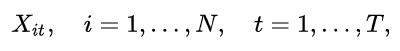
\includegraphics[width=\textwidth]{images/panel.png}
%    \end{subfigure}
%\end{figure}
%
%where $i$ is the individual dimension and $t$ is the time dimension.\vspace{0.5\baselineskip}\\
%
%A general panel data regression model is written as
%
%\begin{figure}
%    \begin{subfigure}[t]{.3\textwidth}
%      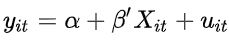
\includegraphics[width=\textwidth]{images/regression.png}
%    \end{subfigure}
%\end{figure}
%
%where
%
%\begin{figure}
%    \begin{subfigure}[t]{.25\textwidth}
%      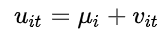
\includegraphics[width=\textwidth]{images/errors.png}
%    \end{subfigure}
%\end{figure}
%
%Estimation with a \textbf{fixed effects} or \textbf{random effects} model depends on assumptions about $\mu_i$, the individual-specific, time-invariant effects.
%
%\end{frame}

%------------------------------------------%
% Takeaway
%------------------------------------------%

\begin{frame}{}

\begin{center}
\begin{minipage}{3.85in}


\includegraphics[width=.25in]{images/prayer.png} {\Large \textbf{Thank you for coming.}}\vspace{0.5\baselineskip}\\

This is the first, albeit crude, open source forecast of cannabis sales in 2022. You can create your own forecasts and see who's model predicts better (based on RMSE)!

\vspace{0.5\baselineskip}

$$
RMSE = \sqrt{\frac{1}{T}\Sigma(Y_{t+1} - \hat{Y}_{t+1})^2}
$$

\end{minipage}
\end{center}

\end{frame}

%------------------------------------------%
% Finale
%------------------------------------------%
\end{document}
